\documentclass[a0paper]{article}
\usepackage[landscape,top=5cm,bottom=3cm,right=5cm,left=5cm]{geometry}
\usepackage{graphicx}
\usepackage[T1]{fontenc}
\usepackage{lmodern}
\usepackage{tikz}
\usepackage{color}
\usepackage{multicol}


\tikzset{
  every overlay node/.style={
    draw=black,fill=white,rounded corners,anchor=north west,
  },
}
% Usage:
% \tikzoverlay at (-1cm,-5cm) {content};
% or
% \tikzoverlay[text width=5cm] at (-1cm,-5cm) {content};
\def\tikzoverlay{%
   \tikz[baseline,overlay]\node[draw=white,every overlay node]
}%

\begin{document}

\begin{tikzpicture}[remember picture,overlay] 
    \node[opacity=1.0] (background) at (current page.center) {
    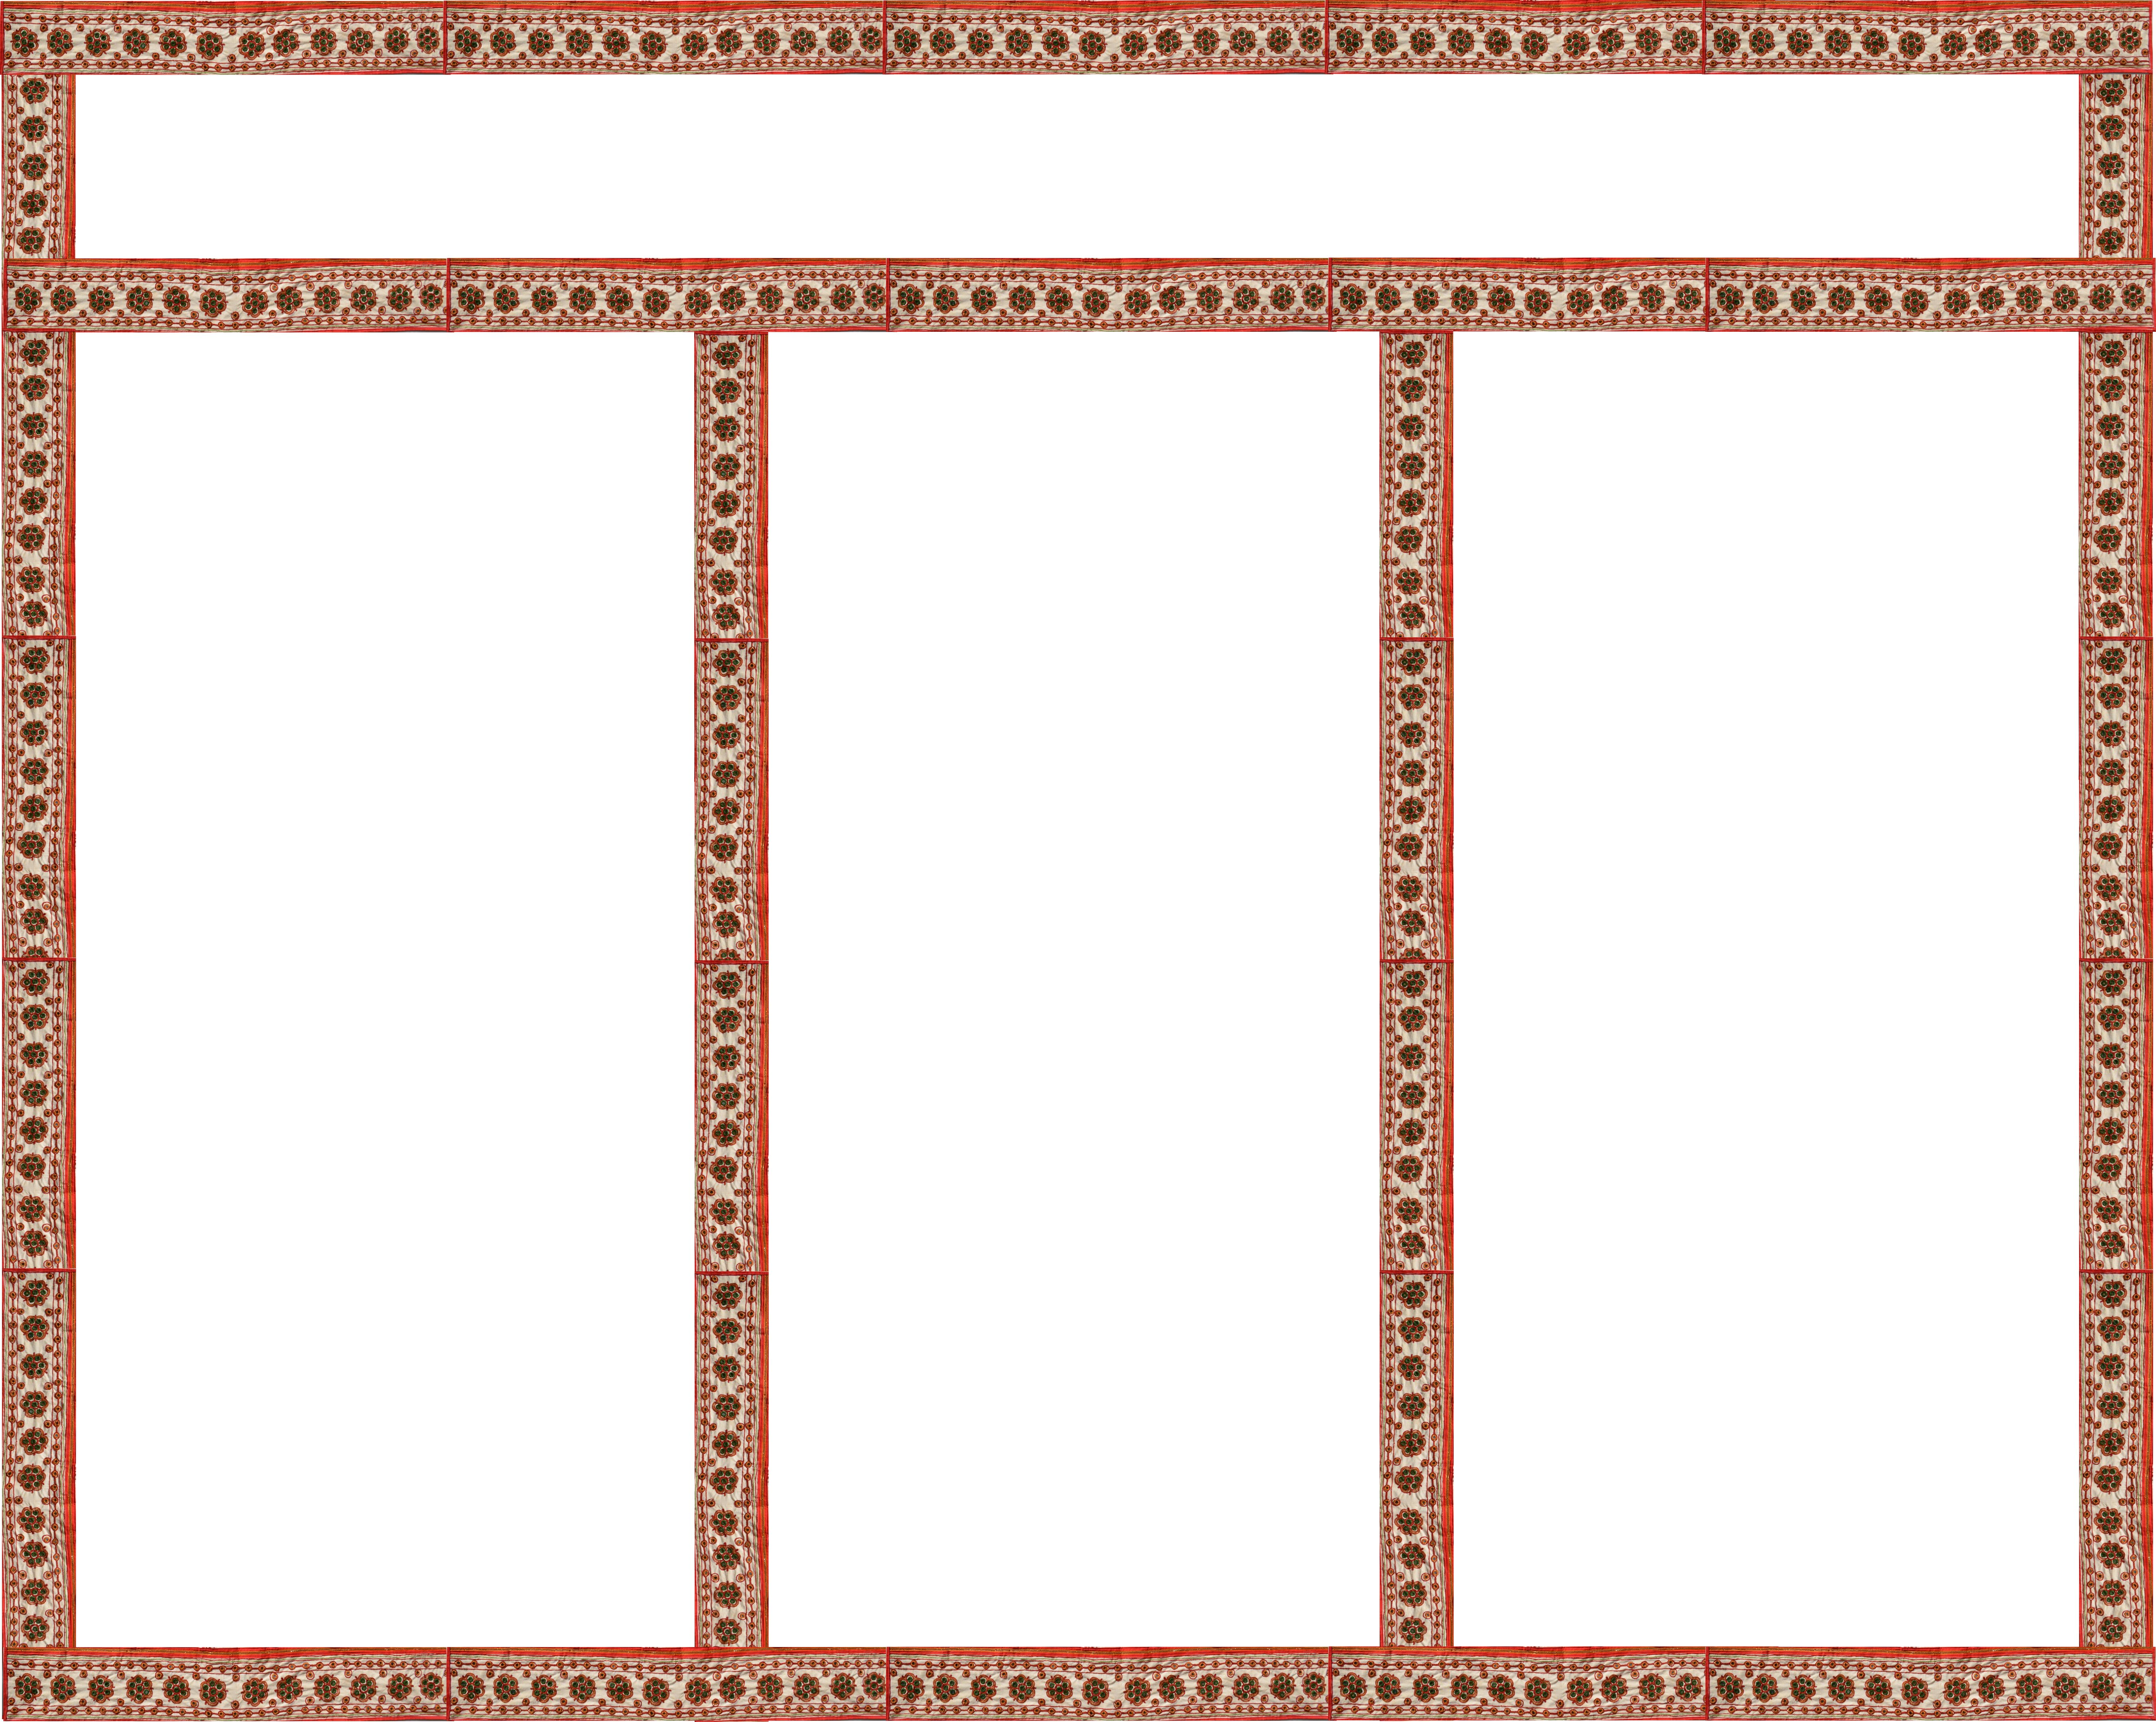
\includegraphics[width=\paperwidth,height=\paperheight]{./background.jpg}
};
\end{tikzpicture}

%%% here goes the title and all
%\tikzoverlay[draw=white,text width=\textwidth] at (10cm,-4cm) {
%    \fontsize{4cm}{1em}\selectfont Modelling Memory Across Scale
%};
%

\begin{minipage}{\textwidth}
    \centering
    \fontsize{4cm}{1em}\selectfont \textcolor{red}{Modelling Memory Across Scale}
    \\
    \fontsize{1.5cm}{1em}\selectfont Aditya Gilra, Aviral Goel, Dilawar Singh,
    Harsha Rani, Sahil Moza, Subhasis Ray, Upinder Bhalla
\end{minipage}


%% Three columns
\vspace{5cm}
\setlength{\columnsep}{6cm}
\begin{multicols}{3}

\Huge

This tutorial is relatively short, largely due to the fact that the whole LaTeX
ethos is concentrate on the content, and let LaTeX (and/or other typographers
who have developed suitable document classes) decide on the best presentation.
The next step to achieve greater control of page layout is to set about
designing your own class. Unfortunately, that is not a straightforward task, and
is often best left to the professionals! 
pIntroduction to multiscale modelling. Here we put a lot of texts and images to
explain the multiscale modeling.  may, therefore, be necessary to manually tweak
the page formatting. Of course, you should only do this at the very final stage
of producing your document, once all the content is complete. LaTeX offers the
following:


Breaks the line at the point of the command.  Breaks the line at the point of
the command, but also stretches the line to the margin. If the optional number
argument is supplied, you convert the command from a demand to a request. The
number must be between 0-4, with 4 being the most insistent.  Ends the current
page Breaks the current page at the point of the command. If the optional number
argument is supplied, you convert the command from a demand to a request. The
number must be between 0-4, with 4 being the most insistent.  Stops the page
being broken at the point of the command. If the optional number argument is
supplied, you convert the command from a demand to a request. The number must be
between 0-4, with 4 being the most insistent.  Ends the current page and causes
any floats encountered in the input, but yet to appear, to be printed.  Summary

This tutorial is relatively short, largely due to the fact that the whole LaTeX
ethos is concentrate on the content, and let LaTeX (and/or other typographers
who have developed suitable document classes) decide on the best presentation.
The next step to achieve greater control of page layout is to set about
designing your own class. Unfortunately, that is not a straightforward task, and
is often best left to the professionals! 
pIntroduction to multiscale modelling. Here we put a lot of texts and images to
explain the multiscale modeling.  may, therefore, be necessary to manually tweak
the page formatting. Of course, you should only do this at the very final stage
of producing your document, once all the content is complete. LaTeX offers the
following:


Breaks the line at the point of the command.  Breaks the line at the point of
the command, but also stretches the line to the margin. If the optional number
argument is supplied, you convert the command from a demand to a request. The
number must be between 0-4, with 4 being the most insistent.  Ends the current
page Breaks the current page at the point of the command. If the optional number
argument is supplied, you convert the command from a demand to a request. The
number must be between 0-4, with 4 being the most insistent.  Stops the page
being broken at the point of the command. If the optional number argument is
supplied, you convert the command from a demand to a request. The number must be
between 0-4, with 4 being the most insistent.  Ends the current page and causes
any floats encountered in the input, but yet to appear, to be printed.  Summary

This tutorial is relatively short, largely due to the fact that the whole LaTeX
ethos is concentrate on the content, and let LaTeX (and/or other typographers
who have developed suitable document classes) decide on the best presentation.
The next step to achieve greater control of page layout is to set about
designing your own class. Unfortunately, that is not a straightforward task, and
is often best left to the professionals! 
pIntroduction to multiscale modelling. Here we put a lot of texts and images to
explain the multiscale modeling.  may, therefore, be necessary to manually tweak
the page formatting. Of course, you should only do this at the very final stage
of producing your document, once all the content is complete. LaTeX offers the
following:


Breaks the line at the point of the command.  Breaks the line at the point of
the command, but also stretches the line to the margin. If the optional number
argument is supplied, you convert the command from a demand to a request. The
number must be between 0-4, with 4 being the most insistent.  Ends the current
page Breaks the current page at the point of the command. If the optional number
argument is supplied, you convert the command from a demand to a request. The
number must be between 0-4, with 4 being the most insistent.  Stops the page
being broken at the point of the command. If the optional number argument is
supplied, you convert the command from a demand to a request. The number must be
between 0-4, with 4 being the most insistent.  Ends the current page and causes
any floats encountered in the input, but yet to appear, to be printed.  Summary

This tutorial is relatively short, largely due to the fact that the whole LaTeX
ethos is concentrate on the content, and let LaTeX (and/or other typographers
who have developed suitable document classes) decide on the best presentation.
The next step to achieve greater control of page layout is to set about
designing your own class. Unfortunately, that is not a straightforward task, and
is often best left to the professionals! 
pIntroduction to multiscale modelling. Here we put a lot of texts and images to
explain the multiscale modeling.  may, therefore, be necessary to manually tweak
the page formatting. Of course, you should only do this at the very final stage
of producing your document, once all the content is complete. LaTeX offers the
following:


Breaks the line at the point of the command.  Breaks the line at the point of
the command, but also stretches the line to the margin. If the optional number
argument is supplied, you convert the command from a demand to a request. The
number must be between 0-4, with 4 being the most insistent.  Ends the current
page Breaks the current page at the point of the command. If the optional number
argument is supplied, you convert the command from a demand to a request. The
number must be between 0-4, with 4 being the most insistent.  Stops the page
being broken at the point of the command. If the optional number argument is
supplied, you convert the command from a demand to a request. The number must be
between 0-4, with 4 being the most insistent.  Ends the current page and causes
any floats encountered in the input, but yet to appear, to be printed.  Summary

This tutorial is relatively short, largely due to the fact that the whole LaTeX
ethos is concentrate on the content, and let LaTeX (and/or other typographers
who have developed suitable document classes) decide on the best presentation.
The next step to achieve greater control of page layout is to set about
designing your own class. Unfortunately, that is not a straightforward task, and
is often best left to the professionals! 
pIntroduction to multiscale modelling. Here we put a lot of texts and images to
explain the multiscale modeling.  may, therefore, be necessary to manually tweak
the page formatting. Of course, you should only do this at the very final stage
of producing your document, once all the content is complete. LaTeX offers the
following:


Breaks the line at the point of the command.  Breaks the line at the point of
the command, but also stretches the line to the margin. If the optional number
argument is supplied, you convert the command from a demand to a request. The
number must be between 0-4, with 4 being the most insistent.  Ends the current
page Breaks the current page at the point of the command. If the optional number
argument is supplied, you convert the command from a demand to a request. The
number must be between 0-4, with 4 being the most insistent.  Stops the page
being broken at the point of the command. If the optional number argument is
supplied, you convert the command from a demand to a request. The number must be
between 0-4, with 4 being the most insistent.  Ends the current page and causes
any floats encountered in the input, but yet to appear, to be printed.  Summary

This tutorial is relatively short, largely due to the fact that the whole LaTeX
ethos is concentrate on the content, and let LaTeX (and/or other typographers
who have developed suitable document classes) decide on the best presentation.
The next step to achieve greater control of page layout is to set about
designing your own class. Unfortunately, that is not a straightforward task, and
is often best left to the professionals! 
pIntroduction to multiscale modelling. Here we put a lot of texts and images to
explain the multiscale modeling.  may, therefore, be necessary to manually tweak
the page formatting. Of course, you should only do this at the very final stage
of producing your document, once all the content is complete. LaTeX offers the
following:


Breaks the line at the point of the command.  Breaks the line at the point of
the command, but also stretches the line to the margin. If the optional number
argument is supplied, you convert the command from a demand to a request. The
number must be between 0-4, with 4 being the most insistent.  Ends the current
page Breaks the current page at the point of the command. If the optional number
argument is supplied, you convert the command from a demand to a request. The
number must be between 0-4, with 4 being the most insistent.  Stops the page
being broken at the point of the command. If the optional number argument is
supplied, you convert the command from a demand to a request. The number must be
between 0-4, with 4 being the most insistent.  Ends the current page and causes
any floats encountered in the input, but yet to appear, to be printed.  Summary

This tutorial is relatively short, largely due to the fact that the whole LaTeX
ethos is concentrate on the content, and let LaTeX (and/or other typographers
who have developed suitable document classes) decide on the best presentation.
The next step to achieve greater control of page layout is to set about
designing your own class. Unfortunately, that is not a straightforward task, and
is often best left to the professionals! 
pIntroduction to multiscale modelling. Here we put a lot of texts and images to
explain the multiscale modeling.  may, therefore, be necessary to manually tweak
the page formatting. Of course, you should only do this at the very final stage
of producing your document, once all the content is complete. LaTeX offers the
following:


Breaks the line at the point of the command.  Breaks the line at the point of
the command, but also stretches the line to the margin. If the optional number
argument is supplied, you convert the command from a demand to a request. The
number must be between 0-4, with 4 being the most insistent.  Ends the current
page Breaks the current page at the point of the command. If the optional number
argument is supplied, you convert the command from a demand to a request. The
number must be between 0-4, with 4 being the most insistent.  Stops the page
being broken at the point of the command. If the optional number argument is
supplied, you convert the command from a demand to a request. The number must be
between 0-4, with 4 being the most insistent.  Ends the current page and causes
any floats encountered in the input, but yet to appear, to be printed.  Summary

This tutorial is relatively short, largely due to the fact that the whole LaTeX
ethos is concentrate on the content, and let LaTeX (and/or other typographers
who have developed suitable document classes) decide on the best presentation.
The next step to achieve greater control of page layout is to set about
designing your own class. Unfortunately, that is not a straightforward task, and
is often best left to the professionals! 
p

\end{multicols}

\end{document}
